% !TEX encoding = UTF-8 Unicode
% !TEX root = ../main.tex
% !TEX spellcheck = en-US

\chapter{Results}
In this chapter, we present the results of this study. 
In this study, we evaluated the design and software quality of the system. This study also addresses all of the research questions. 


%No documentation for pattern usage, but they have a document with coding standard. This includes how to use some patterns. But no docs on where patterns are used, not so big focus on it. 

%Hvor mye er gjenbrukt
%Finne klasser som brukes mye
%Se etter super-klasser
%Memory footprint
%Bruken av C++, gjenbruk kan skape arch drift
%Se etter kode som ikke blir brukt
%Kunne teste ting isolert




\section{Measuring the Software Quality using Metrics}

\subsection{Traditional Metrics}
\label{sub:QA_metrics_results}



\begin{table}[]
\centering
\caption{Project Summary}
\label{tab:projectsummary}
\begin{tabular}{|l|l|l|l|l|}
\hline
                                                    & \textbf{CCCC} & \textbf{SonarQube} & \textbf{Understand}                      & \textbf{SourceMonitor} \\ \hline
\textbf{Lines}                                      &               & 88404              & 88546                                    & 88546                  \\ \hline
\textbf{Lines of Code (LOC)}                        & 46220         & 48693              & 49287                                    &                        \\ \hline
\textbf{Number of Files (NOF)}                      &               & 461                & 461                                      & 461                    \\ \hline
\textbf{Number of Modules (NOM)}                    & 459           &                    &                                          &                        \\ \hline
\textbf{Classes}                                    &               & 851                & 830                                      & 375                    \\ \hline
\textbf{Functions}                                  &               & 3111               & 3589                                     & 812                    \\ \hline
\textbf{Statements}                                 &               & 45153              & 30109 (executable) + 18882 (declarative) & 35622                  \\ \hline
\textbf{Comments (COM)}                             & 19705         & 15962              & 23017                                    & 22845                  \\ \hline
\textbf{Information Flow Measure (inclusive) (IF4)} & 171493        &                    &                                          &                        \\ \hline
\textbf{Information Flow Measure (visible) (IF4v)}  & 166589        &                    &                                          &                        \\ \hline
\textbf{Information Flow Measure (concrete) (IF4c)} & 3789          &                    &                                          &                        \\ \hline
\end{tabular}
\end{table}


Table \ref{tab:projectsummary} summarizes the measurements over the project as a whole from the different tools. The results from the different tools reveals some differences in the measurements. For example, CCCC did not identify number of files in the project, but instead it identified number of non-trivial modules in the project. Non-trivial modules include all classes, and any other module for which member functions are identified. Furthermore, SonarQube identified 851 classes in the project. We can see that the difference between the results of amount of classes from SourceMonitor/Understand and SonarQube is big. In addition, SonarQube identified a total of 45153 statements in the source code, while Understand identified 35254 statements, which is pretty close to what SourceMonitor identified. 

Using CCCC, we were able to measure information flow between the different modules. This is done by identifying and counting inter-module couplings in the module interfaces. 

%MVG: A measure of the decision complexity of the function which make up the program. The strict definition if this measure is that it is the umber of linearly independent routes through a directed acyclic graph which maps the flow of control of a subprogram. The analyzer counts this by recording the number of distinct decision outcomes contained within each function, which yields a good approximation to the formally defined version of the measure.

%L_C : Lines per comment: Indicates density of comments with respect to logical complexity of program

%M_C: Indicates density of comments with respect to logical complexity of the program.

%IF4: Measure of information flow between modules suggested by Henry and Kafura. The analyzer makes an approx. count of this by counting inter-module couplings identified in the module interfaces.


Moreover, we gathered two types of metrics: Class metrics and file metrics. File metrics returns software quality metrics for the specific file, while class metrics contains metrics for each class. A file can contain multiple classes. We wish to look at the different metrics on each file to indicate if there is any weaknesses in that particular file and what classes the file contains. The metrics we measured are lines of code, complexity of file, average complexity per function, amount of functions, and max depth. 

SonarQube class metric includes nested classes, enums, interfaces, and annotations. Understand and SourceMonitor class metric includes classes and struct keyword. 

SonarQube has more accurate data on classes and functions, while SourceMonitor has more accurate data about statements. 



%Metrics for files:
%- Component / Filename
%- Lines of Code
%- Complexity
%- Complexity per function
%- Structure (classes, methods, statements)
%- Functions


% Skal til Research Method


















\subsection{Object-Oriented Metrics in Firmus}
In addition to the traditional metrics, we have also gathered data using object-oriented metrics. Traditional software metrics are important for identifying large and complex files, but they alone may not tell us why some classes are large and complex. Object-oriented metrics we have used to measure the quality of the code is mostly based on the work of Chidamber and Kemerer.\cite{chidamber1994metrics}. They have proposed a set of static metrics that are designed to measure the quality of object-oriented software. These metrics are widely known, and their metrics suite is the deepest research in object-oriented metrics investigation and the measurements we have are the following: Weighted Method per Class (WMC), Depth of Inheritance Tree (DIT), Number of Children (NOC), Lack of Cohesion in Methods (LCOM), Response For a Class (RFC), and Coupling between Object Classes (CBO). In addition to these metrics, we have chosen to count the number of instance variables and instance methods in each class. These values can help us identifying Large Class code smell. 


A description of object-oriented metrics can be found in Chapter 3, Section X. 


\subsection{Object-Oriented Metrics for the whole Project}
 We have decided to exclude the tests from object-oriented metrics analysis. A total of 321 files were analyzed. These files contains 229 classes, and 32068 lines of code. Descriptive statistics such as minimum, maximum, median, sample mean, and standard deviation are presented in this section. Table \ref{tab:oometrics-firmus} presents descriptive statistics for class level metrics for the whole project.

\begin{table}[]
\centering
\caption{OO-metrics for Project Firmus}
\label{tab:oometrics-firmus}
\begin{tabular}{|l|l|l|l|l|l|}
\hline
\textbf{Metric} & \textbf{Min} & \textbf{Max} & \textbf{Median} & \textbf{Sample Mean} & \textbf{Standard Deviation} \\ \hline
LCOM            & 0            & 100          & 55              & 42.205               & 33.042                      \\ \hline
DIT             & 0            & 4            & 1               & 1.061                & 1.062                       \\ \hline
CBO             & 0            & 30           & 5               & 6.079                & 5.179                       \\ \hline
NOC             & 0            & 20           & 0               & 0.454                & 1.850                       \\ \hline
RFC             & 0            & 115          & 10              & 15.777               & 18.677                      \\ \hline
WMC             & 0            & 48           & 7               & 8.616                & 7.167                       \\ \hline
NIM             & 0            & 48           & 7               & 8.376                & 6.983                       \\ \hline
NIV             & 0            & 18           & 1               & 2.223                & 2.811                       \\ \hline
WMC2            & 0            & 325          & 10              & 19.707                 & 31.391                      \\ \hline
\end{tabular}
\end{table}

TODO: Find X\% of the total classes with high coupling, low cohesion, deep hierarchy. 

\textbf{LCOM}: A class is cohesive if LCOM is low. The median shows that more than 50\% of the classes have low cohesion. Classes with low cohesion increases the complexity of the software, and may therefore increase the likelihood of errors during development. 

\textbf{DIT and NOC}: DIT value is generally low in the captured statistics. A class with DIT = 0 is the root of a class hierarchy. With an average value of 1, more than half of the classes inherits from a superclass. However, the the max value of DIT indicates some classes with deep hierarchy. Both samle mean of NOC and DIT are pretty low. They show that inheritance is used in most of the classes to an optimal level. This depth level is well managed at this point, and it probably comes from inheritance. However, the median value of NOC points out that that approximately half of the classes have a flat class structure, indicating inheritance may not be used enough. Moreover, the max value of NOC is very large. Classes with high NOC value are difficult to modify, and they usually require more testing because of the effects on changes on all the children. 

\textbf{CBO}: In general, higher values of CBO indicates fault prone classes. Both sample mean and median shows low CBO values for over half of the classes in this system. However, the maximum value that has been captured is very large. This class is an example of a class that is hard to understand, harder to reuse, and more difficult to maintain. 

\textbf{RFC and WMC}: The RFC statistics reveals that most classes have a RFC of less than 10. However, the maximum value is revealed to be 115. Classes with large RFC tends to be complex and have decreased understandability. Testing classes with large RFC is more complicated. In addition, most of the classes have a WMC of less than 7, but there are a few classes with more extreme values. Those classes with highest WMC are candidates for inspection and refactoring. 

\textbf{WMC2} WMC2 is sum of complexity in this class. The majority of the classes have small WMC values. The median values indicates that half of the classes have WMC value of 10 or less. The maximum value of WMC is set to 325. "Two percent of the classes have WMC value more than 100". However, there are a few classes with WMC greater than 100. Classws with high WMC are candidates for 

\textbf{NIM and NIV}: NIM and NIV can help us identify Large Class code smell. The results show that most classes are small. The sample mean of NIV tells us that each class has an average of 2 instance variables. However, the max value reported is 18, indicating that there is at least one class that contains 18 instance variables. The sample mean of NIM show us that each class has an average of 8 instance methods. The maximum value is 48, which indicates that at least one class contains 48 methods. These values can help us identifying Large Class code smell.

Maximum number


%Good refactoring would be to look at all the classes and see where we could use more abstraction. Reducing redundancy would reduce code size and speed. 

\subsection{Object-Oriented Metrics for the Components}
Descriptive statistics in Table \ref{tab:oometrics-firmus} reveals statistics for class level metrics for the whole project. However, the statistics does not say anything about class level metrics in the different components. Some of the components may have good object-oriented metric values, while other components have bad statistics. In order to identify weak components, we calculated descriptive statistics for each component. 

\subsubsection{Component A}
Component A contains 56 files. Among these files, we identified 40 classes and 6286 lines of code. Figure \ref{fig:algraph} visualizes the frequency distribution of the analyzed object-oriented metrics. Table \ref{tab:oometrics-al} presents common descriptive statistics of the metric distribution.

\begin{table}[]
\centering
\caption{OO-metrics for component A}
\label{tab:oometrics-al}
\begin{tabular}{|l|l|l|l|l|l|}
\hline
\textbf{Metric} & \textbf{Min} & \textbf{Max} & \textbf{Median} & \textbf{Sample Mean} & \textbf{Standard Deviation} \\ \hline
LCOM            & 0            & 94           & 57              & 42.925               & 35.222                      \\ \hline
DIT             & 0            & 4            & 1               & 1.525                & 1.132                       \\ \hline
CBO             & 0            & 29           & 5               & 5.875                & 6.252                       \\ \hline
NOC             & 0            & 8            & 0               & 0.7                  & 1.652                       \\ \hline
RFC             & 2            & 115          & 28.5            & 40.525               & 32.252                      \\ \hline
WMC             & 2            & 44           & 10.5            & 12.675               & 9.339                       \\ \hline
NIM             & 2            & 40           & 10              & 12.3                 & 8.979                       \\ \hline
NIV             & 0            & 12           & 1               & 2.4                  & 2.889                       \\ \hline
WMC2            & 2            & 194          & 17              & 28.9                 & 35.968                      \\ \hline
\end{tabular}
\end{table}

The DIT values indicate that inheritance hierarchies is somehow flat. Classes with flat inheritance hierarchy usually hints that reuse through inheritance is not used. There are approximately eight classes with flat intheritance hierarchy. Rest of the classes inherits for at least one class. The max value captured show that some classes have deep hierarchy. Higher values for DIT indicates higher degree of reuse, but as tradeoff, it may increase complexity of the class. Moreover, the results indicate that most classes only have a few subclasses. Thirty-two classes has no subclasses. However, one class has NOC value of eight. 

The results show that 37.5\% (i.e. 15 classes) of all classes are strongly cohesive. This indicates that more than half of the classes show lack of cohesion. By examining Figure \ref{fig:algraph}, we see that two classes has LCOM values larger than 90\%, indicating loose class structures. Furthermore, most classes have small CBO values, indicating that most classes are self-contained. However, the frequency distribution shows that few of the classes are strongly coupled. One class have CBO value of twenty-nine, indicating a possible fault-prone class which affects its reusability and maintainability. 

The results show that each class have at least two methods. More than half of the classes have low RFC values, which indicates greater polymorphism. However, there are few classes in this component that has more high RFC. The maximum RFC is 115, and classes with high RFC are usually difficult to maintain and test. 

Moreover, the results reveals that, while most classes have a WMC of less than ten, there are few classes with WMC greater than 40. These classes are primary candidates for inspection as they affect many other objects. 

NIM and NIV values indicates that most classes have few instance variables and methods. 

Classes with lage number of instance variables are few. More than half of the classes has one instance variable or less. The largest number of instance variables is 12, revealing that software system does not apply information hiding principle approprately for this class. Furthermore, each class is revealed to have two instance methods. Approximately 50\% of the classes have 10 instance methods or less. This means that rest of the classes have more than 10 instance methods, indicating that classes may provide several services to other classes. The maximum value of NIM captured is 40, indicating a possible Large Class code smell. 

\begin{landscape}
\setlength\LTleft{-.5in}
	\begin{figure}
	\label{fig:algraph}
	\caption{Frequency distribution of OO-metrics in Component A}
	\centering
	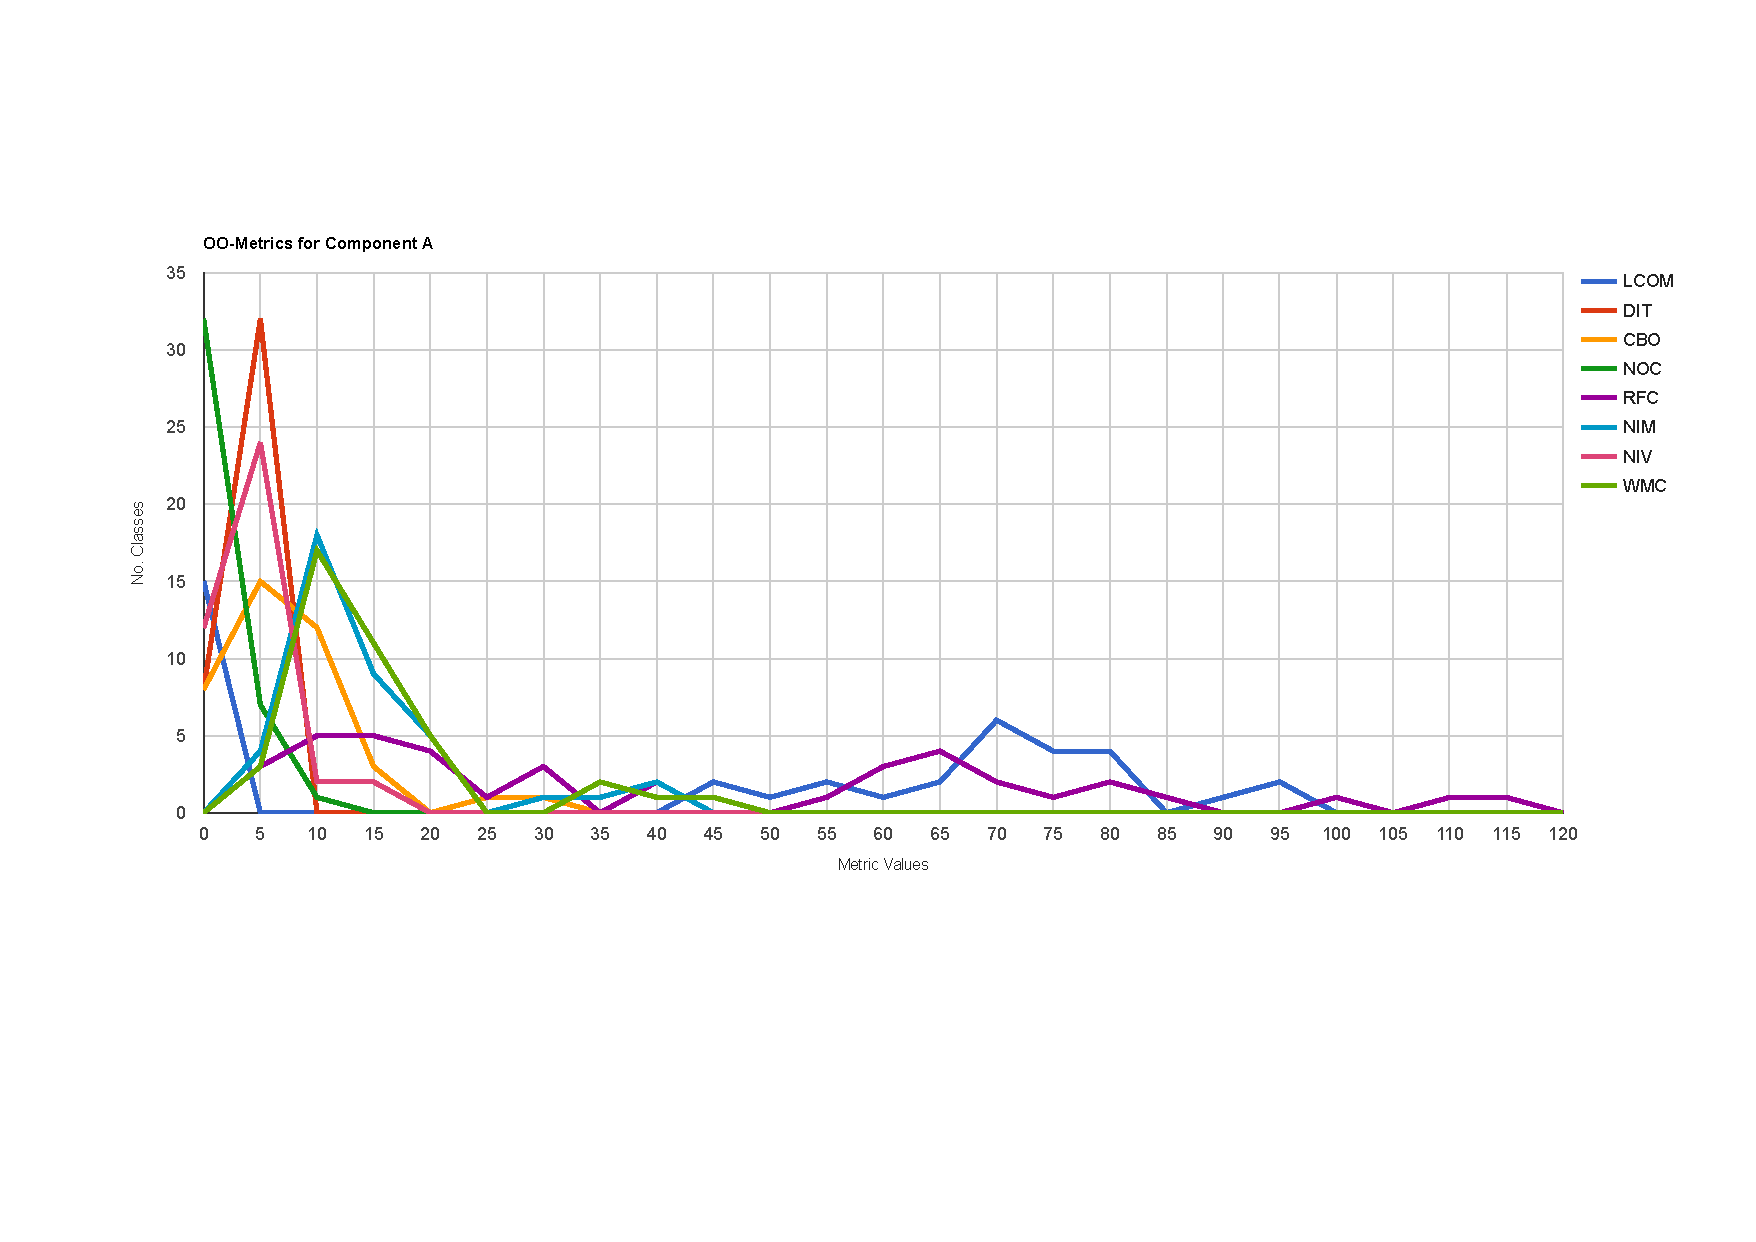
\includegraphics[width=\textwidth]{images/al.pdf}
	\end{figure}
\end{landscape}





\subsubsection{Component B}
We identified 23 classes in Component B. These classes are spread across 42 files. Component B has 3905 LOC. Figure \ref{fig:blcgraph} presents a frequency chart of the object-oriented metric results for Component B. Table \ref{tab:oometrics-blc} presents descriptive statistics of the metric distribution.


\begin{table}[]
\centering
\caption{OO-metrics for Component B}
\label{tab:oometrics-blc}
\begin{tabular}{|l|l|l|l|l|l|}
\hline
\textbf{Metric} & \textbf{Min} & \textbf{Max} & \textbf{Median} & \textbf{Sample Mean} & \textbf{Standard Deviation} \\ \hline
LCOM            & 0            & 100          & 55              & 42.205               & 33.042                      \\ \hline
DIT             & 0            & 4            & 1               & 1.061                & 1.061                       \\ \hline
CBO             & 0            & 30           & 5               & 6.079                & 5.179                       \\ \hline
NOC             & 0            & 20           & 0               & 0.454                & 1.850                       \\ \hline
RFC             & 0            & 115          & 10              & 15.777               & 18.677                      \\ \hline
WMC             & 0            & 48           & 7               & 8.616                & 7.156                       \\ \hline
NIM             & 0            & 48           & 7               & 8.375                & 6.983                       \\ \hline
NIV             & 0            & 86           & 1               & 2.222                & 2.811                       \\ \hline
WMC2            & 3            & 325          & 20              & 37.696               & 66.466                      \\ \hline
\end{tabular}
\end{table}

LCOM is very high. Similar to Component A, half of the classes have low cohesion. 

DIT and NOC has a very low sample mean and median. However, max NOC value is 20.

RFC has average values, but max is very high. 

CBO is average, but max value is set to 30.

WMC is average, but max is high. 

NIM and NIV. 

\begin{landscape}
\setlength\LTleft{-.5in}
	\begin{figure}
	\label{fig:blcgraph}
	\caption{Frequency distribution of OO-metrics in Component B}
	\centering
	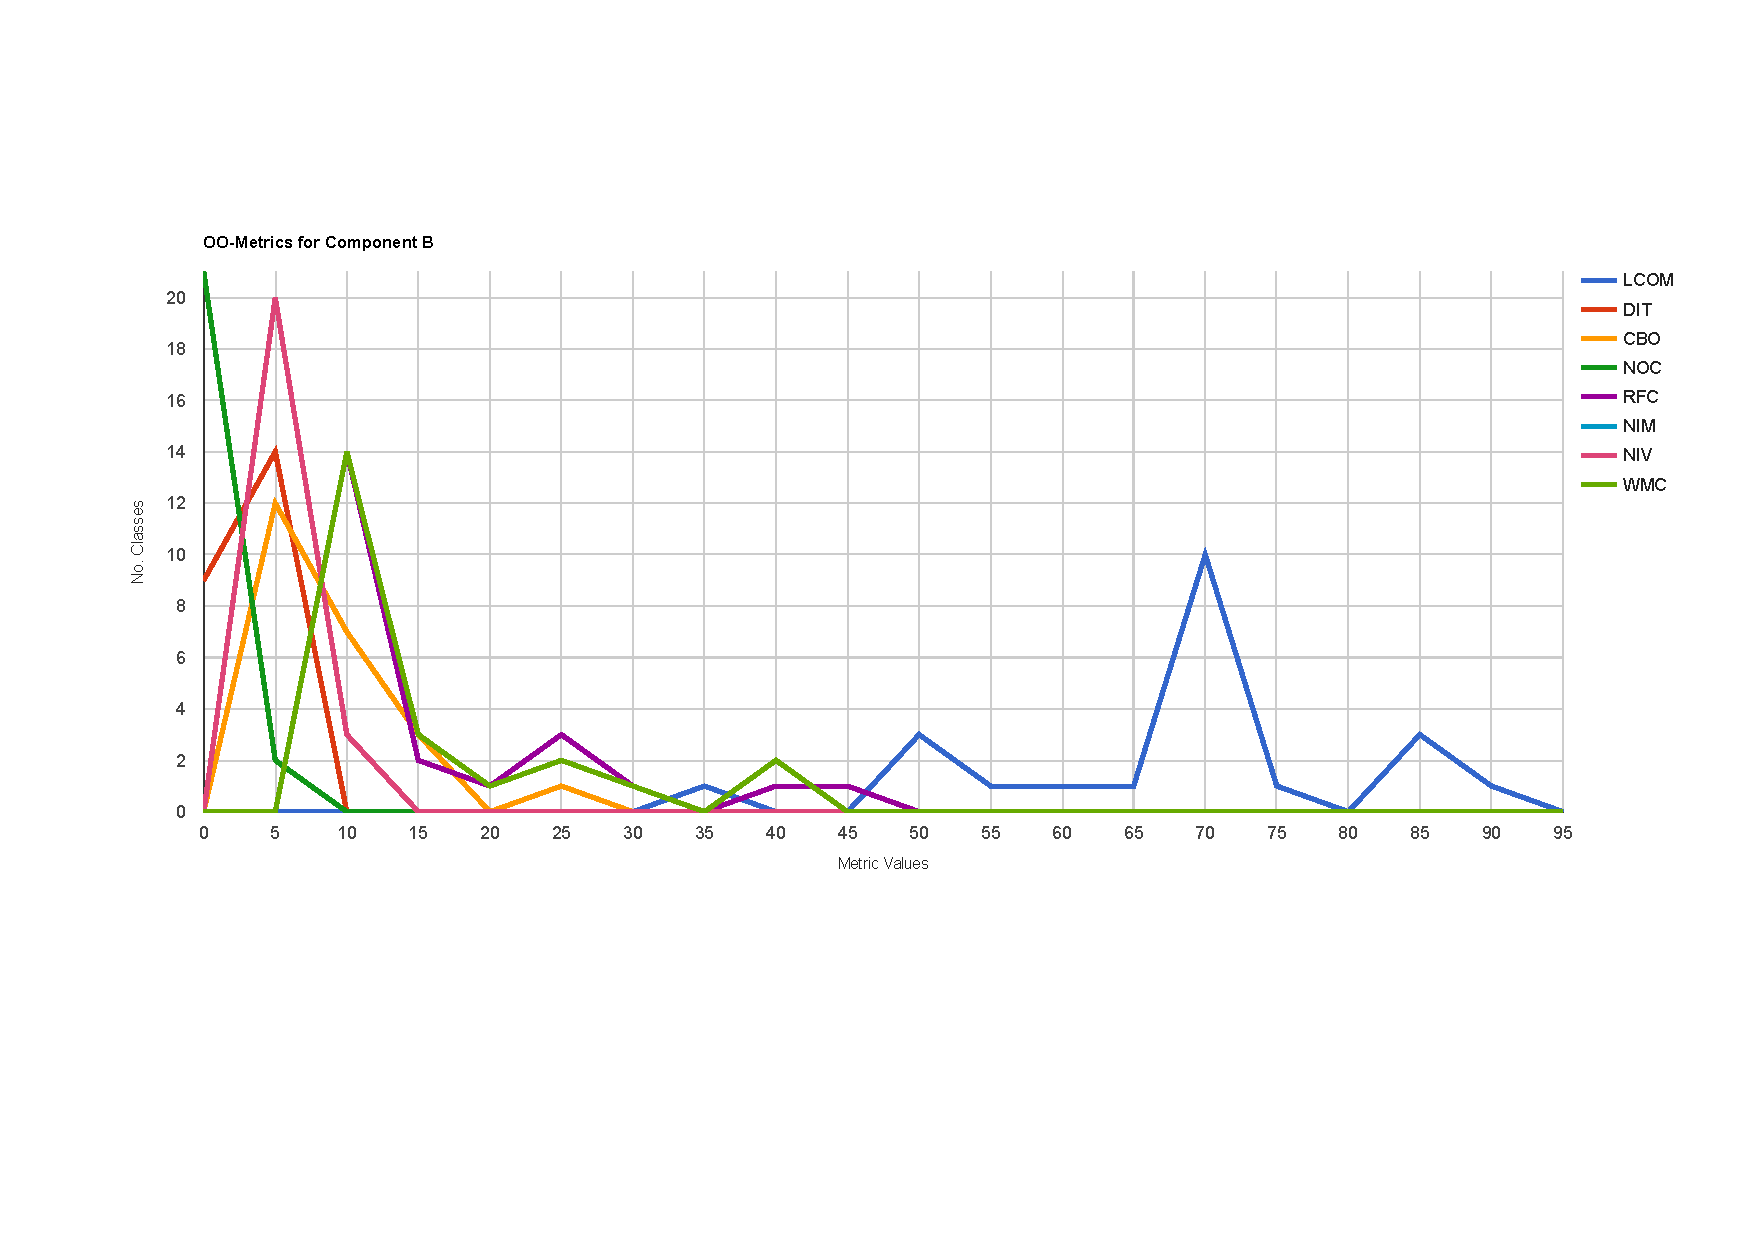
\includegraphics[width=\textwidth]{images/blc.pdf}
	\end{figure}
\end{landscape}






\subsubsection{Component C}
Component C contains 30 files, 20 classes, and 4763 lines of code. 



\begin{landscape}
\setlength\LTleft{-.5in}
	\begin{figure}
	\centering
	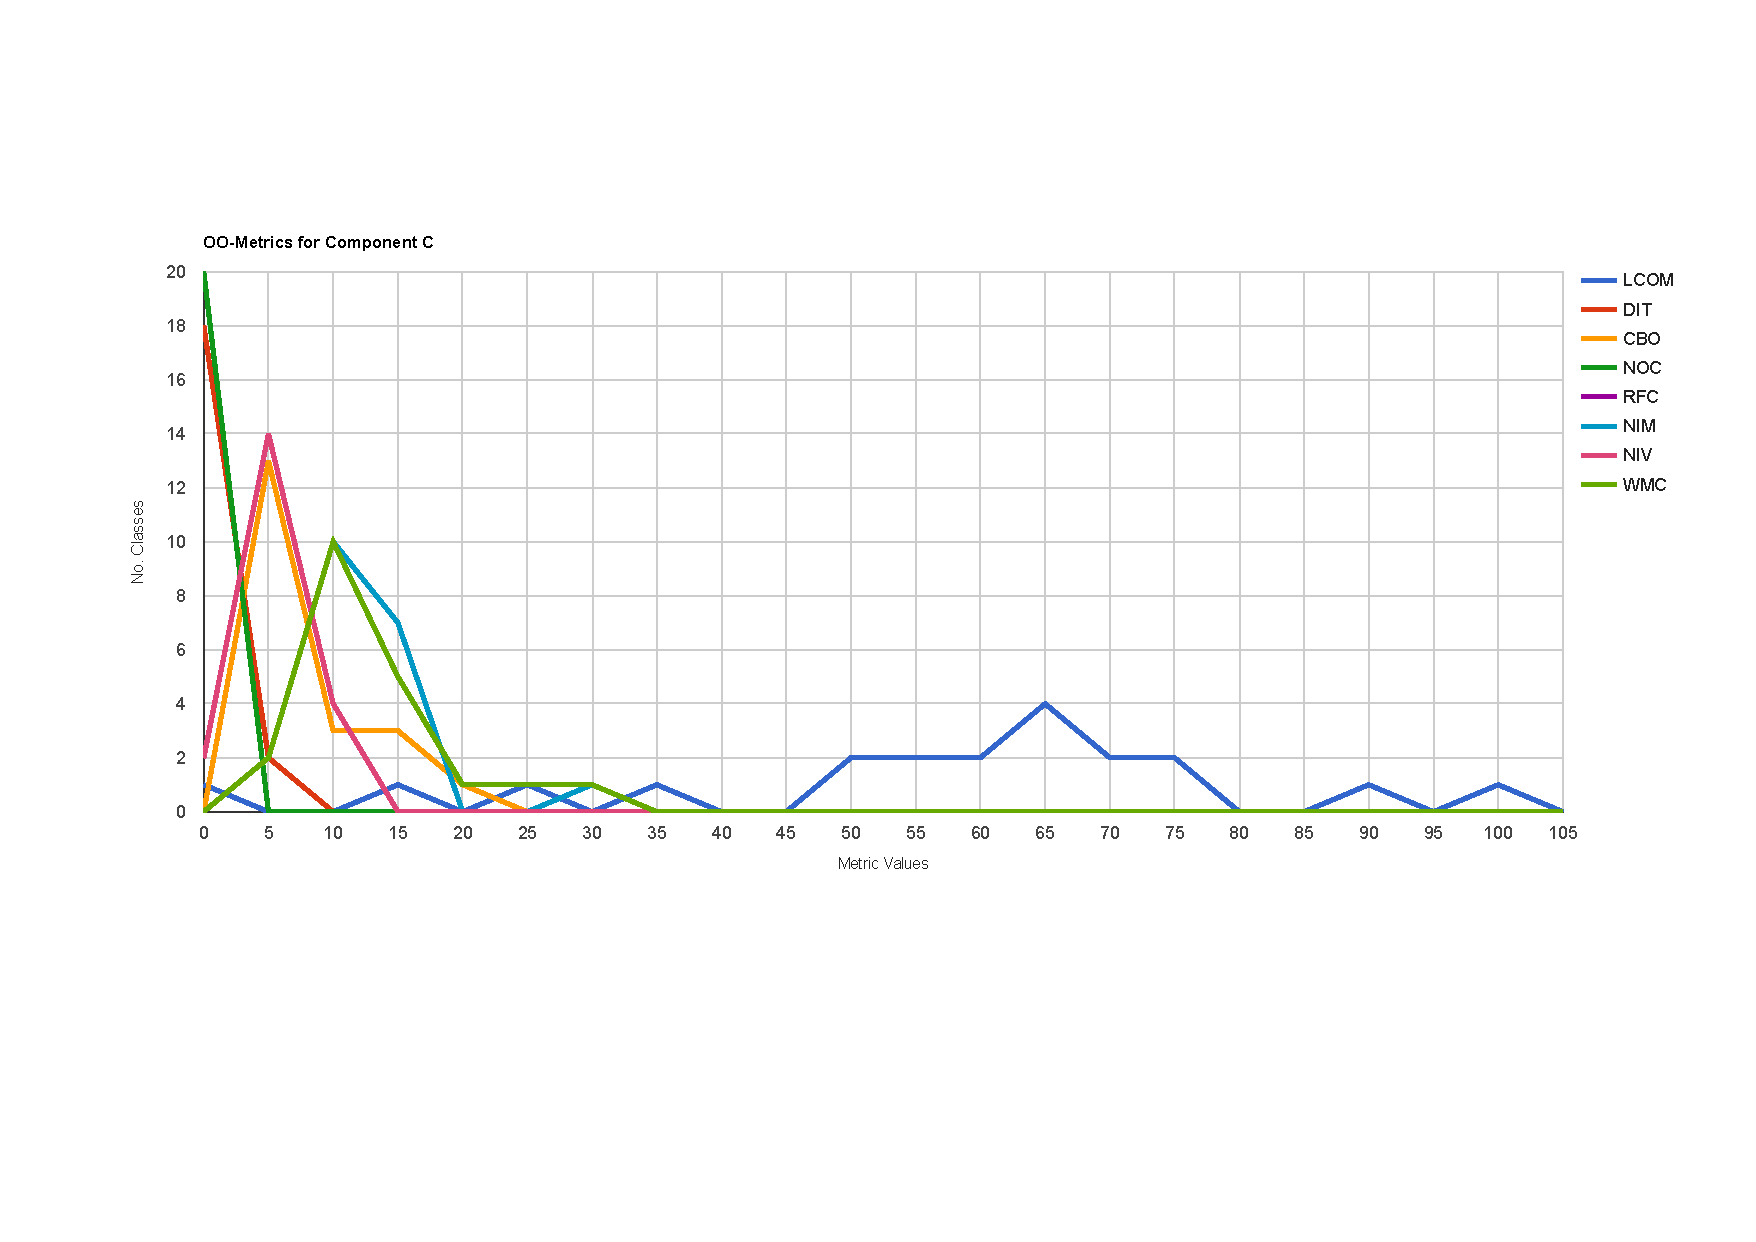
\includegraphics[width=\textwidth]{images/conf.pdf}
	\end{figure}
\end{landscape}



\begin{table}[]
\centering
\caption{OO-metrics for Component C}
\label{tab:oometrics-config}
\begin{tabular}{|l|l|l|l|l|l|}
\hline
\textbf{Metric} & \textbf{Min} & \textbf{Max} & \textbf{Median} & \textbf{Sample Mean} & \textbf{Standard Deviation} \\ \hline
LCOM            & 0            & 99           & 61              & 55.7                 & 23.58                       \\ \hline
DIT             & 0            & 1            & 0               & 0.1                  & 0.308                       \\ \hline
CBO             & 1            & 18           & 4               & 5.55                 & 4.662                       \\ \hline
NOC             & 0            & 0            & 0               & 0                    & 0                           \\ \hline
RFC             & 3            & 26           & 8.5             & 10.3                 & 5.741                       \\ \hline
WMC             & 3            & 26           & 8.5             & 10.3                 & 5.741                       \\ \hline
NIM             & 3            & 26           & 8.5             & 9.85                 & 5.153                       \\ \hline
NIV             & 0            & 9            & 2               & 3.15                 & 3.013                       \\ \hline
WMC2            & 2            & 106          & 9              & 23.25                 & 27.733                      \\ \hline
\end{tabular}
\end{table}

LCOM median shows that half of the classes has more than 60\% LCOM. 

DIT and NOC is very low. Inheritance is not used that much. 

CBO has moderate values, but maximum value is relatively high. 

RFC moderate values.

WMC: Max is a bit far away from sample mean and average.

NIM and NIV






\subsubsection{Component D}
Our analysis show that Component D consists of 13 files and 1647 lines of code. Among these files, we identified only one class. This class has LCOM value of 68, which tells that the class is not very cohesive. DIT value is 1, while NOC is 0. CBO is set to 7, which means that this class is coupled with 7 other modules. RFC, WMC, and NIM is set to 8, meaning that all methods are public and local. The class however has only 1 instance varable. The sum of complexity in this class is 17, which is very low. 



\subsubsection{Component En}
Just like Component D, we identified only one class among 3 files and 367 lines of code. The metrics are very similar to Component D metrics. LCOM value is 62, CBO is 1, NIV is 2 and WMC2 is 15. 





\subsubsection{Component Ex}
48 files, 4089 lines of code. 86 classes.

\begin{table}[]
\centering
\caption{OO-metrics for Component Ex}
\label{tab:oometrics-ex}
\begin{tabular}{|l|l|l|l|l|l|}
\hline
\textbf{Metric} & \textbf{Min} & \textbf{Max} & \textbf{Median} & \textbf{Sample Mean} & \textbf{Standard Deviation} \\ \hline
LCOM            & 0           & 100          & 0               & 25.988               & 32.905                      \\ \hline
DIT             & 0            & 3            & 2               & 1.581                & 1.121                       \\ \hline
CBO             & 0            & 16           & 4               & 4.919                & 4.018                       \\ \hline
NOC             & 0            & 20           & 0               & 0.744                & 2.736                       \\ \hline
RFC             & 0            & 28           & 8               & 10.279               & 6.030                       \\ \hline
WMC             & 0            & 22           & 3.5             & 5.07                 & 3.928                       \\ \hline
NIM             & 0            & 22           & 3               & 4.907                & 3.846                       \\ \hline
NIV             & 0            & 10           & 0               & 1.209                & 2.098                       \\ \hline
WMC2            & 0            & 41          & 7              & 8.744                 & 8.117                      \\ \hline
\end{tabular}
\end{table}


\begin{landscape}
\setlength\LTleft{-.5in}
	\begin{figure}
	\label{fig:exgraph}
	\caption{Coming}
	\centering
	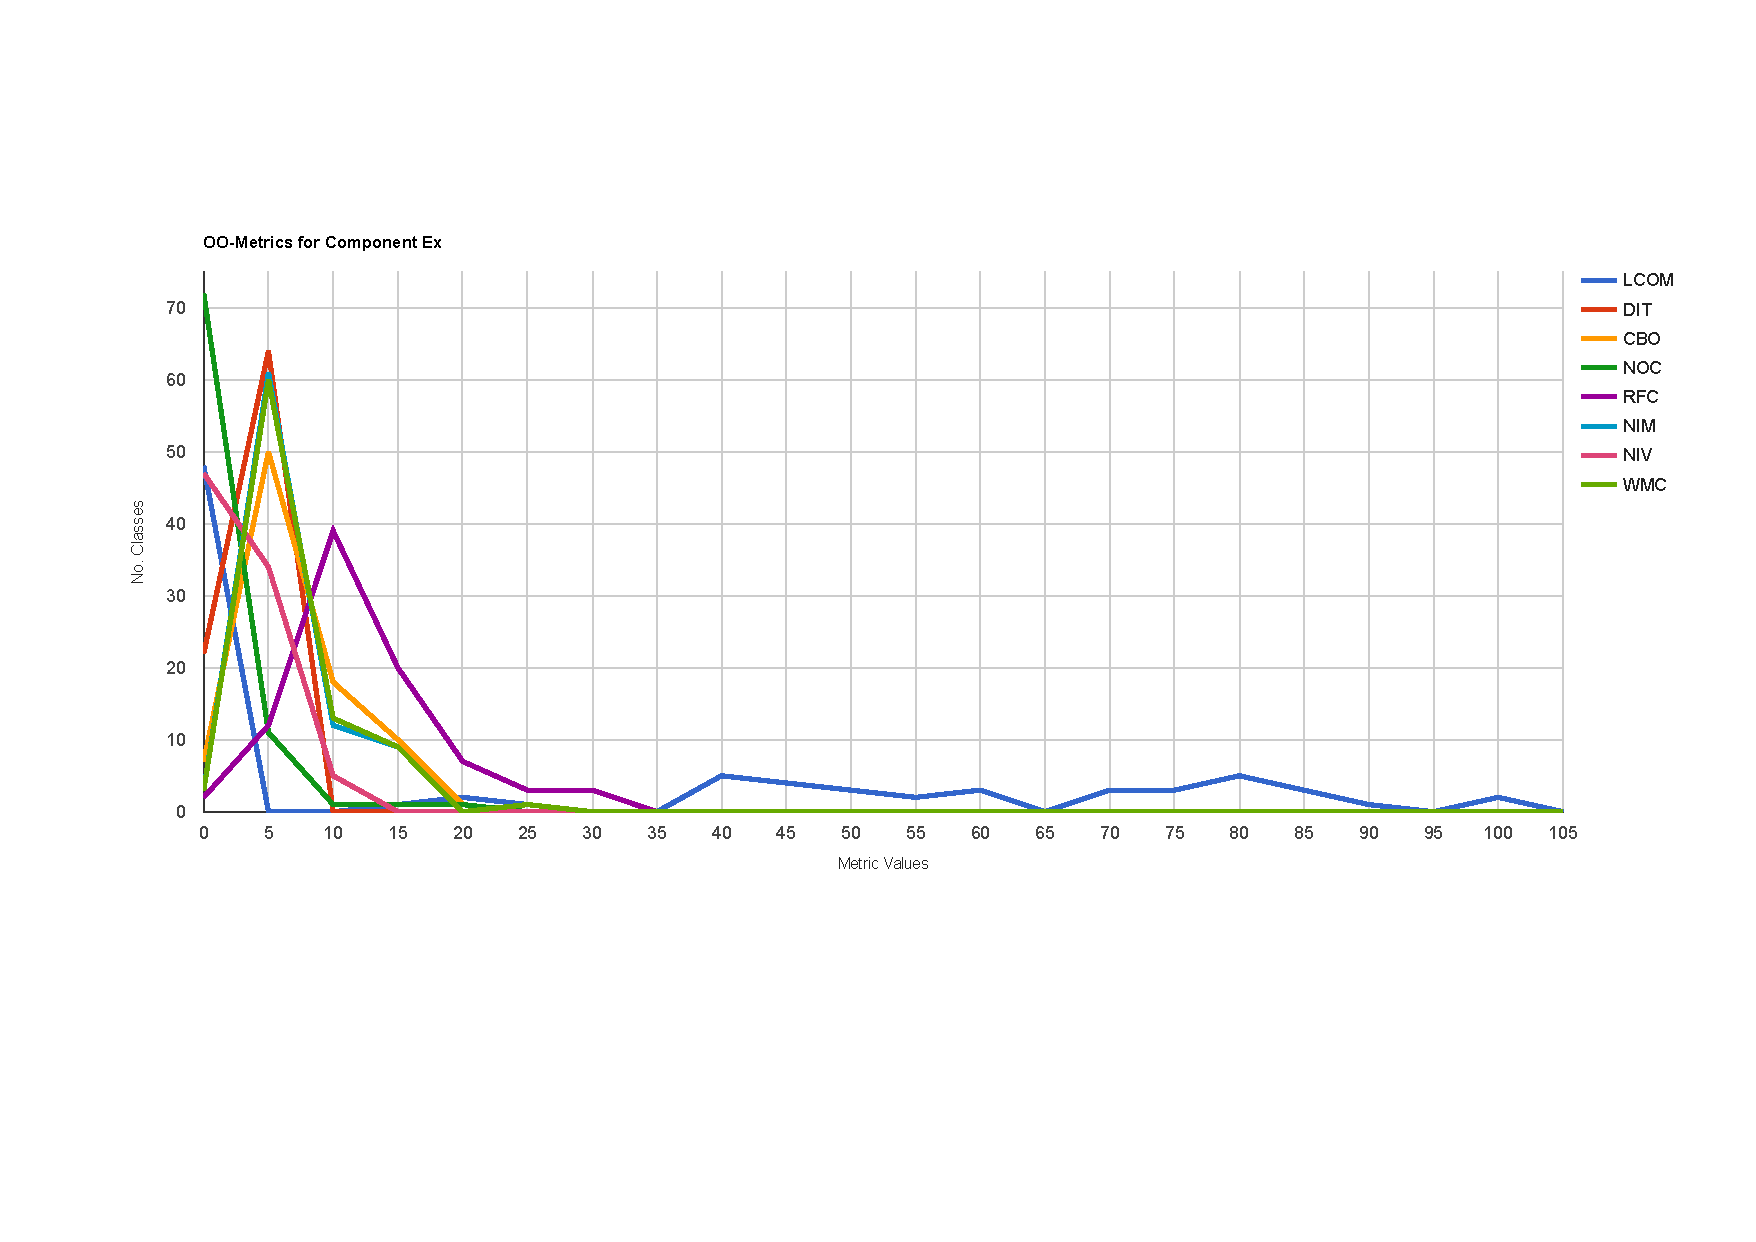
\includegraphics[width=\textwidth]{images/ex.pdf}
	\end{figure}
\end{landscape}







\subsubsection{Component G}
59 files, 3701 lines of code, 32 classes.


\begin{table}[]
\centering
\caption{Component G}
\label{tab:oometrics-guri}
\begin{tabular}{|l|l|l|l|l|l|}
\hline
\textbf{Metric} & \textbf{Min} & \textbf{Max} & \textbf{Median} & \textbf{Sample Mean} & \textbf{Standard Deviation} \\ \hline
LCOM            & 0            & 94           & 60              & 50.25                & 31.236                      \\ \hline
DIT             & 0            & 2            & 1               & 0.625                & 0.609                       \\ \hline
CBO             & 0            & 22           & 5.5             & 6.187                & 4.987                       \\ \hline
NOC             & 0            & 2            & 0               & 0.25                 & 0.622                       \\ \hline
RFC             & 2            & 30           & 9               & 10.187               & 6.382                       \\ \hline
WMC             & 2            & 30           & 7.5             & 8.594                & 5.405                       \\ \hline
NIM             & 0            & 29           & 7               & 8.437                & 5.459                       \\ \hline
NIV             & 0            & 18           & 2               & 3.062                & 3.926                       \\ \hline
WMC2            & 1            & 123          & 12              & 19.437                 & 24.794                      \\ \hline
\end{tabular}
\end{table}

\begin{landscape}
\setlength\LTleft{-.5in}
	\begin{figure}
	\label{fig:gurigraph}
	\caption{Coming}
	\centering
	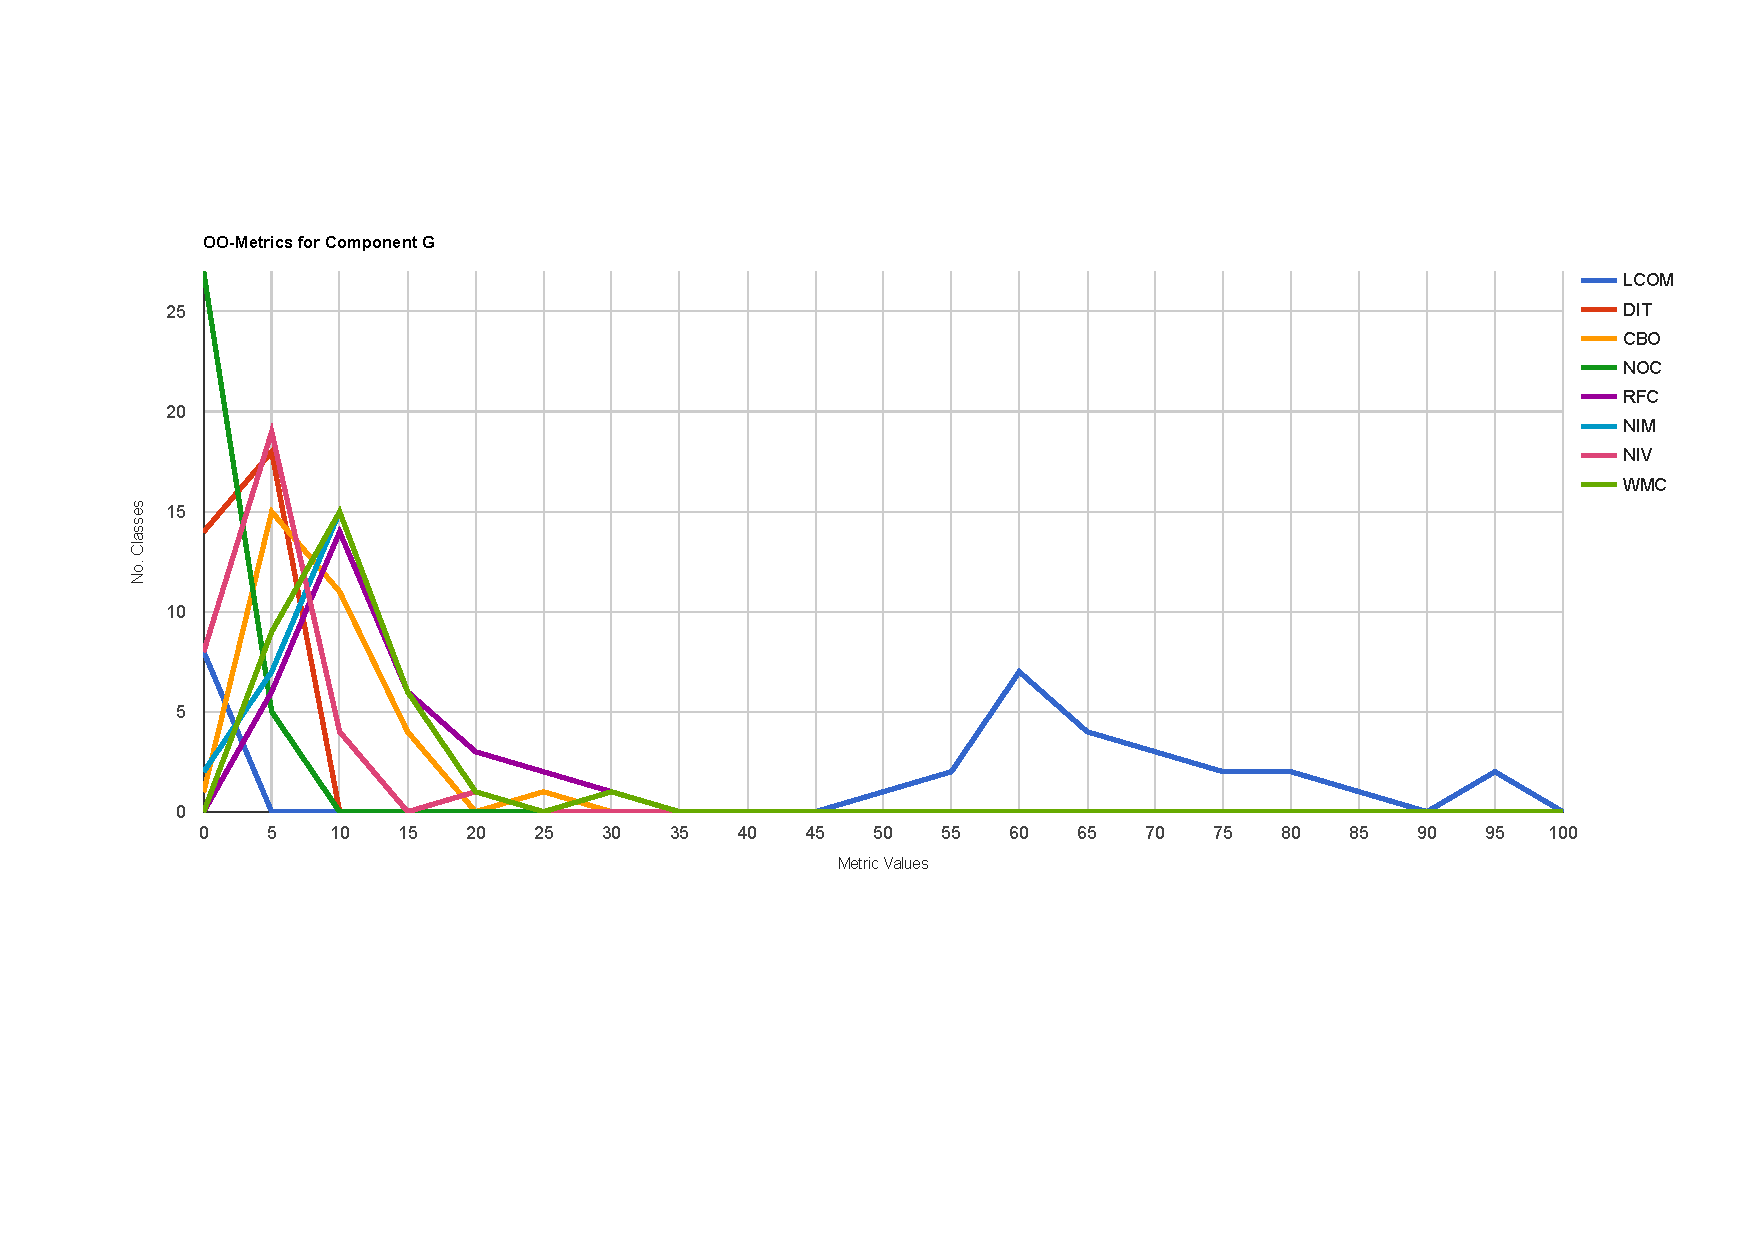
\includegraphics[width=\textwidth]{images/guri.pdf}
	\end{figure}
\end{landscape}





\subsubsection{Component L}
16 files, 849 lines of code, 7 classes.

\begin{table}[]
\centering
\caption{OO-metrics for Component L}
\label{tab:oometrics-log}
\begin{tabular}{|l|l|l|l|l|l|}
\hline
\textbf{Metric} & \textbf{Min} & \textbf{Max} & \textbf{Median} & \textbf{Sample Mean} & \textbf{Standard Deviation} \\ \hline
LCOM            & 0            & 80           & 58              & 50.857               & 35.130                      \\ \hline
DIT             & 0            & 1            & 1               & 0.571                & 0.534                       \\ \hline
CBO             & 1            & 13           & 4               & 5.571                & 4.197                       \\ \hline
NOC             & 0            & 0            & 0               & 0                    & 0                           \\ \hline
RFC             & 5            & 12           & 9               & 8.571                & 2.936                       \\ \hline
WMC             & 5            & 12           & 9               & 8.571                & 2.936                       \\ \hline
NIM             & 3            & 12           & 7               & 8.286                & 3.402                       \\ \hline
NIV             & 0            & 5            & 1               & 1.571                & 2.070                       \\ \hline
WMC2            & 4            & 42          & 11              & 19.571                 & 14.524                      \\ \hline
\end{tabular}
\end{table}



\begin{landscape}
\setlength\LTleft{-.5in}
	\begin{figure}
	\label{fig:loggraph}
	\caption{Coming}
	\centering
	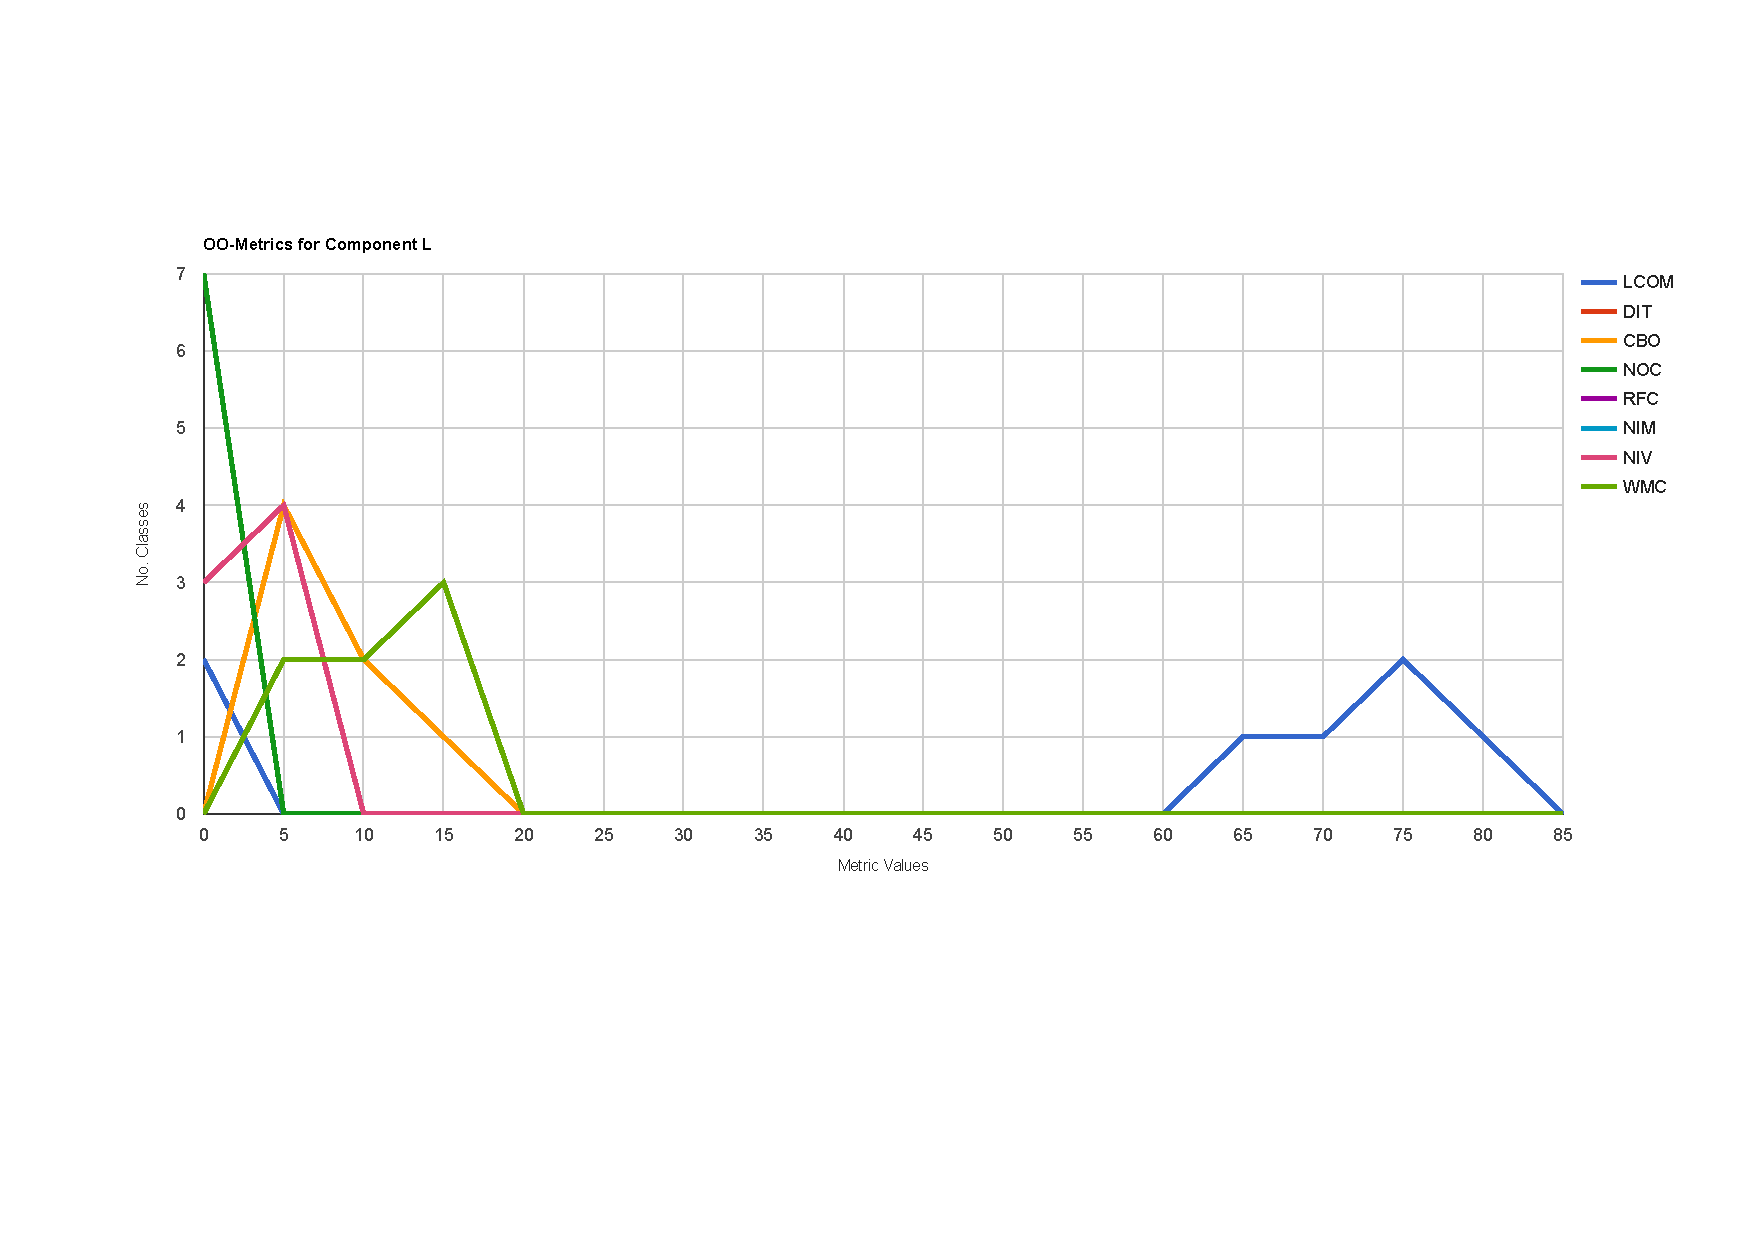
\includegraphics[width=\textwidth]{images/log.pdf}
	\end{figure}
\end{landscape}







\subsubsection{Component N}
17 files, 1839 lines of code, 8 classes.

\begin{table}[]
\centering
\caption{OO-metrics for Component N}
\label{tab:oometrics-netw}
\begin{tabular}{|l|l|l|l|l|l|}
\hline
\textbf{Metric} & \textbf{Min} & \textbf{Max} & \textbf{Median} & \textbf{Sample Mean} & \textbf{Standard Deviation} \\ \hline
LCOM            & 0            & 79           & 70.5            & 54.5                 & 33.899                      \\ \hline
DIT             & 0            & 1            & 0               & 0.25                 & 0.463                       \\ \hline
CBO             & 3            & 17           & 10.5            & 10                   & 4.140                       \\ \hline
NOC             & 0            & 1            & 0               & 0.125                & 0.353                       \\ \hline
RFC             & 6            & 32           & 9               & 11.625               & 8.568                       \\ \hline
WMC             & 6            & 23           & 9               & 10.5                 & 5.580                       \\ \hline
NIM             & 6            & 21           & 8.5             & 9.75                 & 5.036                       \\ \hline
NIV             & 0            & 8            & 5.5             & 4.375                & 3.068                       \\ \hline
WMC2            & 4            & 125          & 32              & 40.375                 & 36.707                      \\ \hline
\end{tabular}
\end{table}


\begin{landscape}
\setlength\LTleft{-.5in}
	\begin{figure}
	\label{fig:netgraph}
	\caption{Coming}
	\centering
	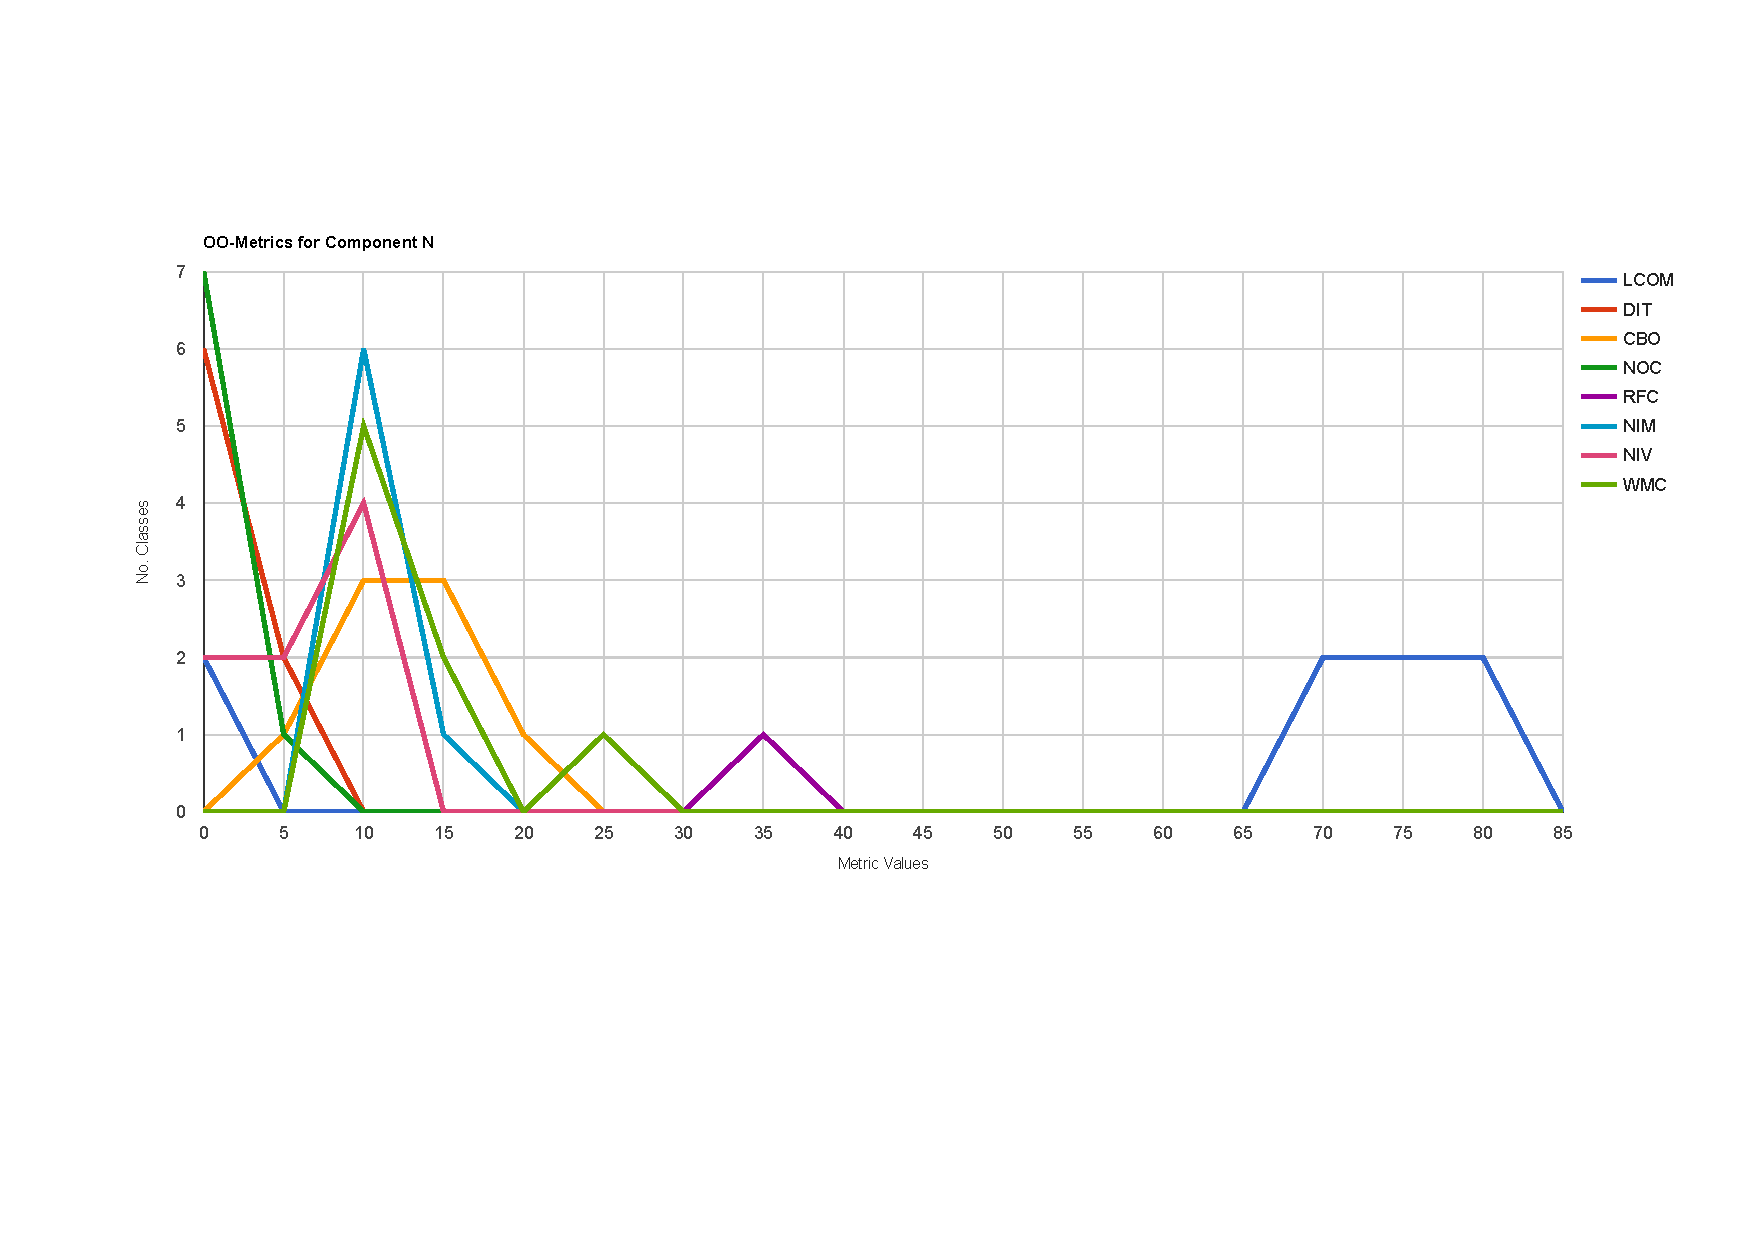
\includegraphics[width=\textwidth]{images/network.pdf}
	\end{figure}
\end{landscape}



\subsubsection{Component P}
12 files, 722 lines of code, 8 classes.



\begin{table}[]
\centering
\caption{OO-metrics for Component P}
\label{tab:oometrics-proc}
\begin{tabular}{|l|l|l|l|l|l|}
\hline
\textbf{Metric} & \textbf{Min} & \textbf{Max} & \textbf{Median} & \textbf{Sample Mean} & \textbf{Standard Deviation} \\ \hline
LCOM            & 0            & 81           & 65              & 58.25                & 26.611                      \\ \hline
DIT             & 0            & 1            & 0               & 0.25                 & 0.463                       \\ \hline
CBO             & 0            & 12           & 5.5             & 5.5                  & 3.964                       \\ \hline
NOC             & 0            & 1            & 0               & 0.125                & 0.353                       \\ \hline
RFC             & 2            & 14           & 6.5             & 7.5                  & 3.625                       \\ \hline
WMC             & 2            & 14           & 6.5             & 7.25                 & 3.412                       \\ \hline
NIM             & 2            & 13           & 6.5             & 7                    & 3.117                       \\ \hline
NIV             & 0            & 6            & 3.5             & 3.125                & 2.031                       \\ \hline
WMC2            & 1            & 47           & 8               & 15.75                & 15.809                      \\ \hline
\end{tabular}
\end{table}



\begin{landscape}
\setlength\LTleft{-.5in}
	\begin{figure}
	\label{fig:procgraph}
	\caption{Coming}
	\centering
	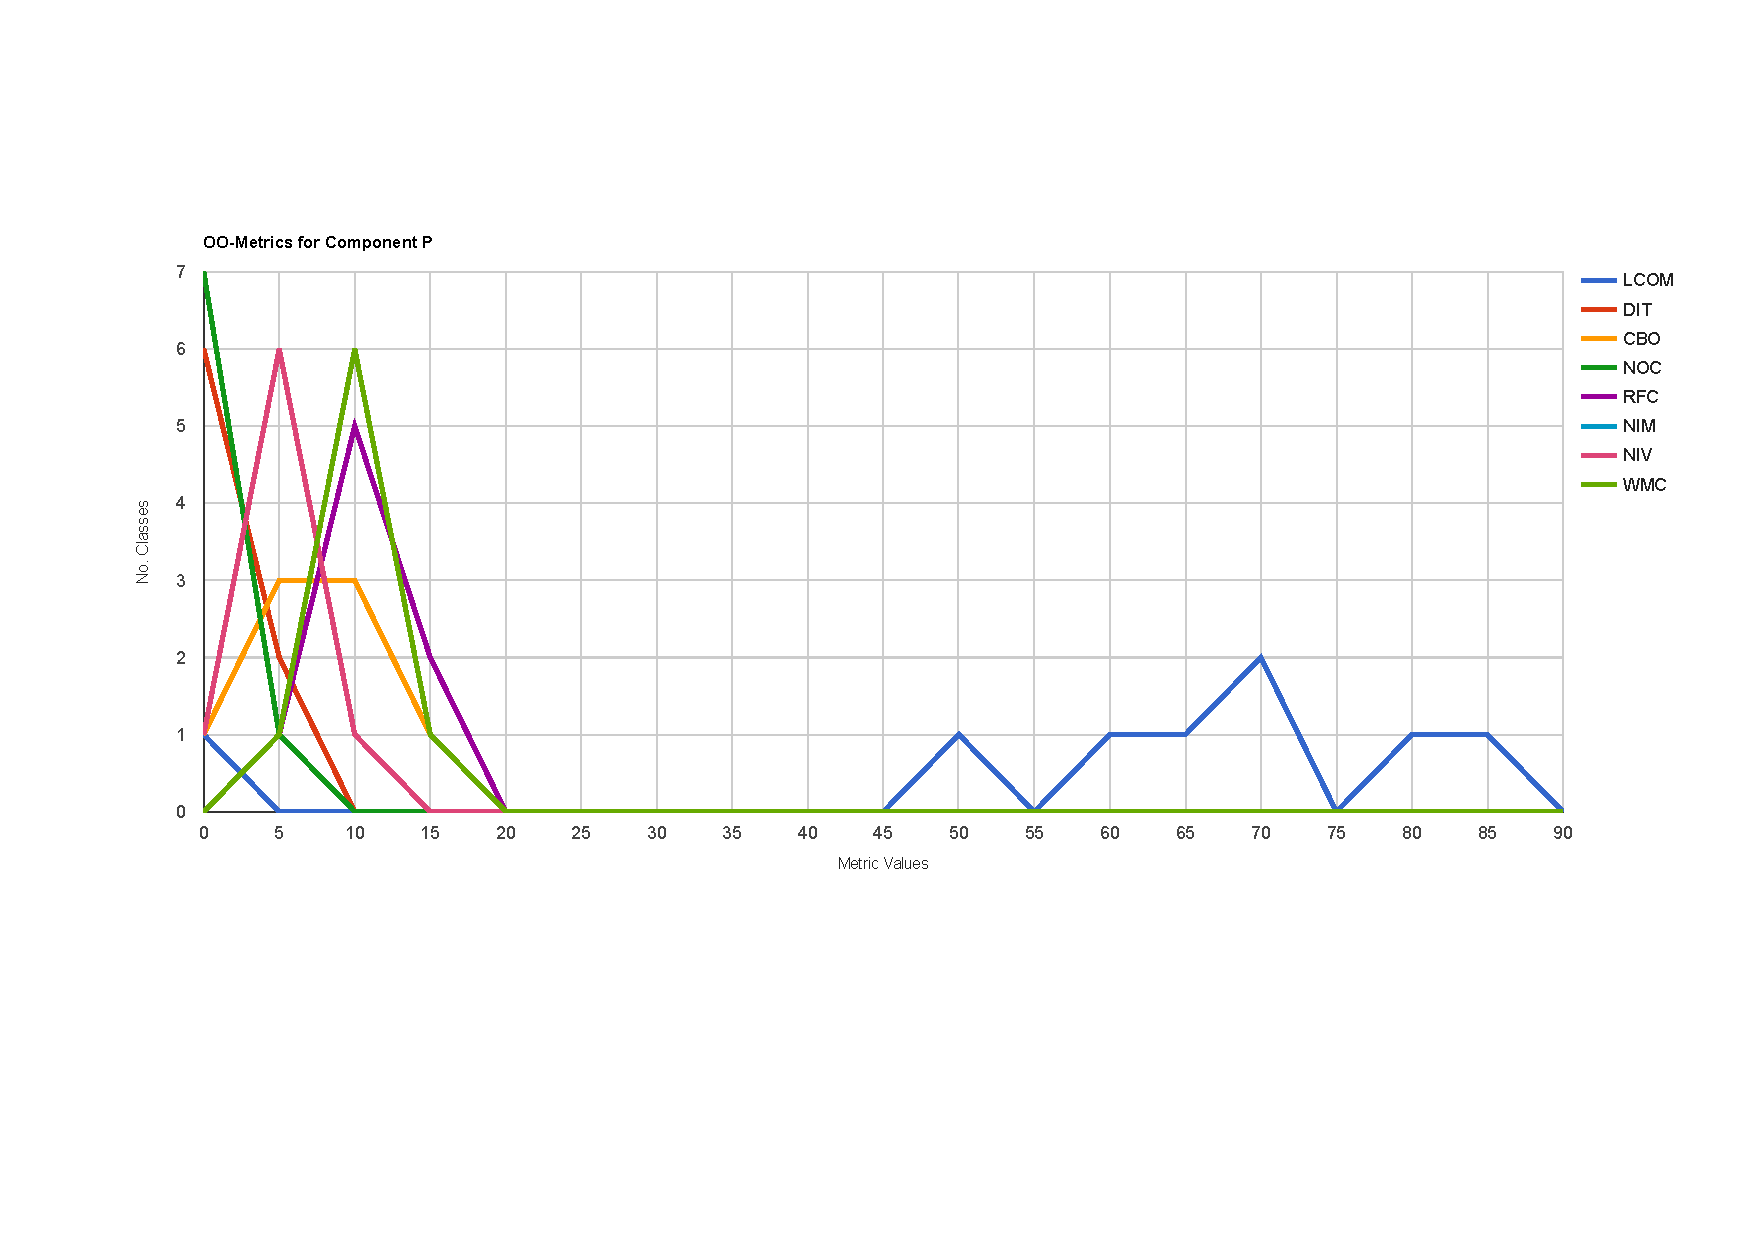
\includegraphics[width=\textwidth]{images/process.pdf}
	\end{figure}
\end{landscape}



\subsubsection{Component S}
4 files, 223 lines of code, 2 classes.
\begin{table}[]
\centering
\caption{OO-metrics for Component S}
\label{tab:oometrics-sys}
\begin{tabular}{|l|l|l|l|l|l|}
\hline
\textbf{Metric} & \textbf{Min} & \textbf{Max} & \textbf{Median} & \textbf{Sample Mean} & \textbf{Standard Deviation} \\ \hline
LCOM            & 33           & 50           & 41.5            & 41.5                 & 12.021                      \\ \hline
DIT             & 0            & 1            & 0.5             & 0.5                  & 0.707                       \\ \hline
CBO             & 3            & 6            & 4.5             & 4.5                  & 2.121                       \\ \hline
NOC             & 0            & 0            & 0               & 0                    & 0                           \\ \hline
RFC             & 6            & 9            & 7.5             & 7.5                  & 2.121                       \\ \hline
WMC             & 6            & 9            & 7.5             & 7.5                  & 2.121                       \\ \hline
WMC2            & 6           & 19            & 12.5            & 12.5                 & 9.192                         \\ \hline
NIM             & 6            & 9            & 7.5             & 7.5                  & 2.121                       \\ \hline
NIV             & 1            & 1            & 1               & 1                    & 0                           \\ \hline
\end{tabular}
\end{table}






\subsubsection{Component W}
1 file, 1 class, 69 lines of code. 
Component W contains only one file. This file consists of 69 lines of code, and among these, we identfied one class. This class has LCOM value of 58, DIT and NOC of 0, CBO is 4, NIM, RFC, WMC is 6, WMC2 is 8, and NIV is 2. 



Our results show that (whats good and wrong with these metrics, what can be done). 


% HVA SLAGS METRIKKER ER INTERESSANT, GÅ DYPERE INN PÅ DEM. F.EKS METHODS IN CLASS, HVA SIER DET OSS

% TOO MANY LINES OF CODE? CHECK SINGLE RESPONSBILITY PRINCIPLE, it states that every class or module should have responsbility for a single part of the funcitnaility provided by the software.'








\section{Identifying Code Smells using Automatic Approaches}
\label{sub:code_smell_detection}
As we explained in Chapter 2, one of the ways to identify design debt is to look at the number of code smells in the source code. Table \ref{tab:identifiedCodeSmell} describes the number of code smells that were identified using automatic.

\begin{table}[]
\centering
\caption{Number of Code Smells detected}
\label{tab:identifiedCodeSmell}
\begin{tabular}{|l|l|}
\hline
\textbf{Code Smell}                           & \textbf{Detected}    \\ \hline
Long Method                                   & 10          \\ \hline
Large Class                                   & 8          \\ \hline
Long Parameter List                           & 15          \\ \hline
%Data Clumps                                   & Bloaters          \\ \hline
%Switch Statements                             & O-O Abusers       \\ \hline
%Temporary Field                               & O-O Abusers       \\ \hline
%Refused Bequest                               & O-O Abusers       \\ \hline
%Alternative Classes with Different Interfaces & O-O Abusers       \\ \hline
%Parallel Inheritance Hierarchies              & O-O Abusers       \\ \hline
%Divergent Change                              & Change Preventers \\ \hline
%Shotgun Surgery                               & Change Preventers \\ \hline
%Lazy Class                                    & Dispensables      \\ \hline
%Data Class                                    & Dispensables      \\ \hline
Duplicated Code                               & Approximately 5\% of the source code. 39 files affected.       \\ \hline
Speculative Generality                        & 1153      \\ \hline
Dead Code 									  & 151 \\ \hline
\end{tabular}
\end{table}

\subsubsection{Duplicated Code}
Duplicated code is found by looking for pieces of code that appears at multiple places in the source code, both internally in a file or in another file. A piece of code is considered duplicated if the piece of code contains at least 10 lines of code and occurs at multiple places in the source code. Table \ref{tab:identifiedCodeSmell} reports the number of duplicated code found by SonarQube, expressed as a percentage value. Including the test files, the results show that roughly 5\% of the source code contains duplicated code. This corresponds to 4395 lines of code affecting 39 files across the system. By examining the results, we identified that roughly 54\% of the duplicated code is located in Component A. The other duplicated lines are spread across Component B, N, P, C, D, L, Ex, S, and G. Table \ref summarizes duplication in the various components. 

\begin{table}[]
\centering
\caption{Duplication in Project Firmus}
\label{tab:duplicatedLines}
\begin{tabular}{|l|l|}
\hline
\textbf{Component}			& \textbf{Information} \\ \hline
Component A 				& 12 files, 2400 LOC \\ \hline
Component B 				& 6 files, 366 LOC \\ \hline
Component C 				& 3 files, 284 LOC \\ \hline
Component D 				& 2 files, 80 LOC \\ \hline
Component Ex 				& 4 files, 305 LOC \\ \hline
Component G 				& 4 files, 311 LOC \\ \hline
Component L 				& 1 file, 30 LOC \\ \hline
Component N 				& 3 files, 301 LOC \\ \hline
Component P 				& 2 files, 124 LOC \\ \hline
Component S 				& 2 files, 194 LOC \\ \hline
\end{tabular}
\end{table}


\subsubsection{Long Method}
Understand considers a Long Method as code smell if lines of code in method exceeds 200 lines. Using Understand, we identified 10 long methods, spread across six different files. 7 of 10 long methods are located in test files. 


\subsubsection{Long Parameter List}
Long Parameter List code smell is detected by comparing the total number of parameters in a method against a fixed threshold. The maximum number of parameters allowed in a method using CppDepend is set to 5. This means that 6 or more parameters in a method are considered as code smell. The results from CppDepend reports 15 hits of Long Parameter List code smell, where 3 hits are considered as critical. A Long Parameter List hit is critical when total of parameters in a method is higher than 8. The largest number of parameters in a method we identified was 12. These results were verified manually by examining the class diagrams for the corresponding methods.

\subsubsection{Speculative Generality}
Speculative Generality is detected by locating unused classes, methods, fields, or parameters. Table \ref{tab:speculativeGenerality} summarizes Speculative Generality code smell that were identified through a code analysis using Understand. The results are divided into the categories unused functions, unused local variables, and unused static globals. 

\begin{table}[]
\centering
\caption{Speculative Generality Results}
\label{tab:speculativeGenerality}
\begin{tabular}{|l|l|}
\hline
\textbf{Category}		& 	\textbf{Hits} \\ \hline
Unused Methods 			&	794  \\ \hline
Unused Local Variables 	& 	346	 \\ \hline
Unused Static Globals 	& 	13	 \\ \hline
\end{tabular}
\end{table}

\subsubsection{Shotgun Surgery}
The results shows that X classes are infected with the Shotgun Surgery code smell. 



\subsubsection{Dead Code}
Fowler and Beck\cite{1999:RID:311424} do not classify dead code as code smell. However, dead code should be classified as a code smell, as it is a quite common problem as it hinders code comprehension and makes the current program structure less obvious\cite{mantyla2003taxonomy}. We examined three types of "Dead Code" code smell in Project Firmus: "Commented Out" Code, Unreachable Code, and Unnecessary Includes in Header Files. In total, we found 151 hits of "Dead Code" code smell, which we have summarized in Table \ref{tab:deadCode}.

\begin{table}[]
\centering
\caption{Dead Code Results}
\label{tab:deadCode}
\begin{tabular}{|l|l|}
\hline
\textbf{Category}		& 	\textbf{Hits} \\ \hline
"Commented Out" Code 			&	67  \\ \hline
Unreachable Code 	& 	10	 \\ \hline
Unnecessary Includes in Header Files 	& 	74	 \\ \hline
\end{tabular}
\end{table}


\subsubsection{Large Class}
We were not able to identify any large classes using automatic tool. However, by counting the number of instances, variables, and methods using object-oriented metrics, we were able to identify some large classes in the system. Table X summarizes Large Class code smells. 


% ANtiåpattern, move down to metrics, point out that possible god classes may be antipatterns.



How did we study the different code smells, the apporach and the results.
The results from Table XX

As we see, there are many code smells detected. We take a closer look at some of the classes; presented in UML diagrams here:




































